\documentclass[12pt]{book}
\usepackage{geometry}                % See geometry.pdf to learn the layout options. There are lots.
\geometry{letterpaper}                   % ... or a4paper or a5paper or ... 
%\geometry{landscape}                % Activate for for rotated page geometry
%\usepackage[parfill]{parskip}    % Activate to begin paragraphs with an empty line rather than an indent
\usepackage{graphicx}
\usepackage{makeidx}
\usepackage{url}

\makeindex

\title{OpenLCB / NMRAnet S-9.7 DevKit Manual}
%\author{The Author}
%\date{}                                           % Activate to display a given date or no date

\begin{document}
\maketitle

\tableofcontents

\chapter{What's all this in the box?}

Here's what you'll find in the box, and a short description of each to help you get started:
\begin{itemize}
\item 3 x Railstars Io V1.0 boards
\item 1 x TCH Technology OpenLCB USB/CAN Interface board
\item 1 x ButtonLED8 v1.0 board
\item TODO cables
\item TODO potentially useful odds and ends
\end{itemize}

The three Railstars Io boards are the heart of TODO. Each board is designed to connect to various features of your layout, and communicate to each other via the included CAT5 cables.

The TODO ButtonLED8 is a tool to help you quickly get the most from the Railstars Io.

The TCH Technology OpenLCB USB/CAN Interface permits you to expand your layout's capabilities by providing a USB interface to connect your home computer.

\chapter{Basic Concepts of OpenLCB / NMRAnet S-9.7}

TODO What is it?

\section{Producer-Consumer model}
\index{producer-consumer model}

\chapter{Connecting the Railstars Io boards}

\begin{figure}[htbp]
\begin{center}
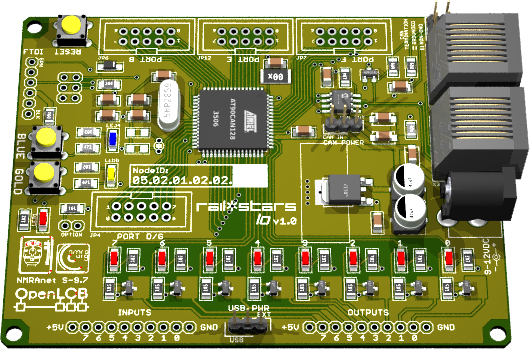
\includegraphics[width=6in]{images/RailstarsIo.png}
\caption{Railstars Io}
\label{Io}
\end{center}
\end{figure}


Railstars Io provides a set of 8 inputs and 8 outputs to connect to your layout. The inputs can be used with the buttons and switches on a fascia panel, or with existing accessories on your layout such as block detectors or turnout feedback units. The outputs can be used directly to control bulbs or LEDs on your layout, or connected to existing accessories on your layout such as turnout controllers or signal decoders.

\section{Initial Setup}

To use Railstars Io, you will first need to solder the appropriate terminals to the input and output banks. You can solder wired directly to the holes in the circuit board, or solder in the included pin headers or screw terminals. If you are unsure which to use, the screw terminals are the most flexible, and will serve most purposes.

\begin{figure}[htbp]
\begin{center}
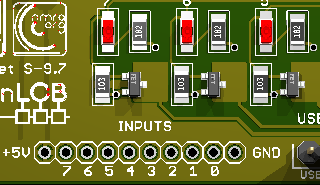
\includegraphics[width=3in]{images/IoInputEmpty.png}
\caption{Railstars Io input bank as shipped}
\label{bareinput}
\end{center}
\end{figure}

\begin{figure}[htbp]
\begin{center}
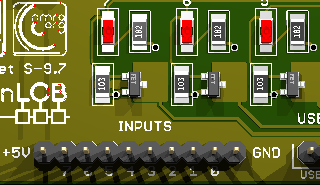
\includegraphics[width=3in]{images/IoInputPinheader.png}
\caption{Railstars Io input bank with pin headers soldered in place}
\label{pinheader}
\end{center}
\end{figure}

\begin{figure}[htbp]
\begin{center}
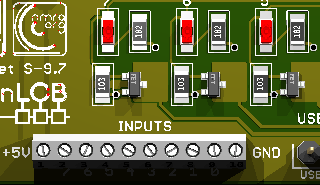
\includegraphics[width=3in]{images/IoInputsWithScrewTerminal.png}
\caption{Railstars Io input bank with screw terminals soldered in place}
\label{screwterminal}
\end{center}
\end{figure}

\section{Connecting to NMRAnet bus}

TODO plug in CAT5 cable. Set termination jumper if needed
TODO images of termination jumpers on and off
\index{NMRAnet!termination}

\section{Providing power}

Railstars Io can be powered in one of three ways: From an external power supply, via the NMRAnet bus, or via a USB connection to a PC.

\subsection{Powering with an external supply}
\label{externalpower}
\index{Railstars Io!power, power adapter}

You may power Railstars Io using an external power supply that provides a 2.1mm center-positive plug, and between 9 and 12V DC at 500mA or more of current. Ensure that the ``USBPWR'' jumper is set to ``EXT'', as per Figure \ref{EXTPWR}

\begin{figure}[htbp]
\begin{center}
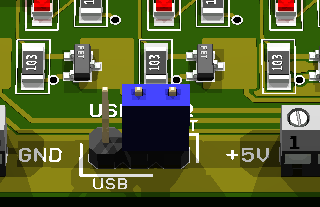
\includegraphics[width=3in]{images/IoUSBPowerEXT.png}
\caption{USBPWR jumper set to external power}
\label{EXTPWR}
\end{center}
\end{figure}

\subsection{Powering via USB}
\index{Railstars Io!power, USB}

Using the included USB cable, you can power Railstars Io via the USB interface. To do so set the ``USBPWR'' jumper is set to ``USB'', as per Figure \ref{USBPWR}, and then plug the USB cable into the FTDI header, following the instructions in \S\ref{FTDI}.

\begin{figure}[htbp]
\begin{center}
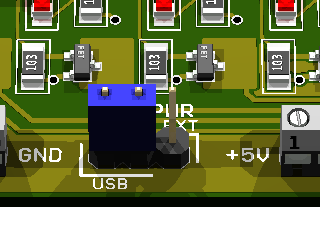
\includegraphics[width=3in]{images/IoUSBPowerUSB.png}
\caption{USBPWR jumper set to USB power}
\label{USBPWR}
\end{center}
\end{figure}

\subsection{Powering via the NMRAnet bus}
\index{Railstars Io!power, NMRAnet from@power, from NMRAnet}
\index{NMRAnet!bus power}

The NMRAnet bus can provide a small amount of power to individual boards. To configure Railstars Io to draw power from the NMRAnet bus, set the ``USBPWR'' jumper to ``EXT'', as per Figure \ref{EXTPWR} above, and then set the ``CAN POWER'' jumper to ``CAN IN'', as per Figure \ref{CANIN}.

\begin{figure}[htbp]
\begin{center}
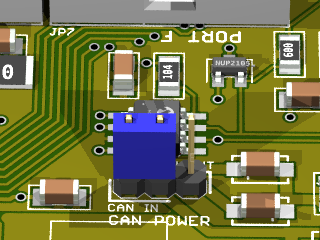
\includegraphics[width=3in]{images/IoCANPowerIn.png}
\caption{CAN POWER jumper set to draw power from the NMRAnet bus}
\label{CANIN}
\end{center}
\end{figure}

Note that drawing power from the NMRAnet bus requires that at least one other node be configured to provide power to the NMRAnet bus.

\subsection{Providing power to the NMRAnet bus}
\index{Railstars Io!power, NMRAnet to@power, to NMRAnet}
\index{NMRAnet!bus power}

A Railstars Io node that is configured to use an external power supply can optionally be configured to provide power to the NMRAnet bus. In this case, a power adapter capable of providing 750mA--1,000mA is suggested. Configure the board as per \S\ref{externalpower}, and then set the ``CAN POWER'' jumper to ``CAN OUT'', as per Figure \ref{CANOUT}.

\begin{figure}[htbp]
\begin{center}
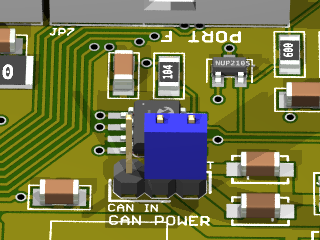
\includegraphics[width=3in]{images/IoCANPowerOut.png}
\caption{CAN POWER jumper set to provide power to the NMRAnet bus}
\label{CANOUT}
\end{center}
\end{figure}

Note: If the Railstars Io will neither draw power from nor provide power to the NMRAnet bus, please remove the ``CAN POWER'' jumper entirely.

\section{Usage Example: ButtonLED8 v1.0}

TODO image of screw terminals and ButtonLED8

\section{Usage Example: Fascia panel}

Railstars Io can be used to interface a fascia panel or control panel to your layout. Simply wire the panel switches to the Io inputs, and the panel indicators to the Io outputs as indicated below. By default, Railstars Io is pre-loaded with a useful configuration for fascia panels, in that each input will trigger the corresponding output; that is, pressing a button wired to input 1 will cause a bulb or LED wired to output 1 to light.

\subsection{Wiring inputs to switches}

Inputs should be wired to short to ground. An open circuit on an input is read as ``off'', and shorting the input to ground is read as ``on''. (It is safe to apply 5V to the inputs, although Io cannot distinguish between an open circuit and +5V on an input line).

Normally-open pushbuttons should be wired as per Figure \ref{pushbutton}, with one leg to the desired input, and the other to ground. In this configuration, a depressed button will be read as ``on''.

\begin{figure}[htbp]
\begin{center}
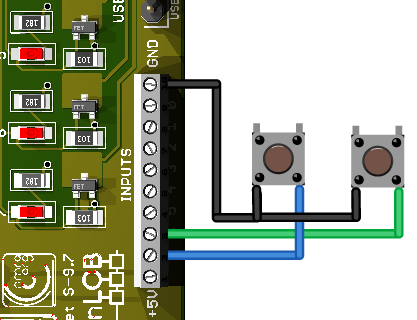
\includegraphics[width=3in]{images/Inputs-pushbutton.png}
\caption{Wiring pushbutton switches to Io inputs}
\label{pushbutton}
\end{center}
\end{figure}

DPDT switches should be wired as per Figure \ref{DPDT}, with the center pin wired to the desired input, one pin wired to ground, and the other left unconnected. In this configuration, moving the toggle towards the wired pin is read as ``on'', and towards the other as ``off''.

\begin{figure}[htbp]
\begin{center}
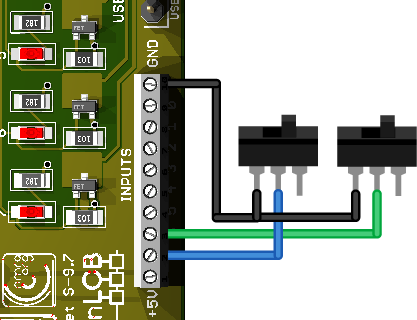
\includegraphics[width=3in]{images/Inputs-DPDT.png}
\caption{Wiring DPDT toggle switches to Io inputs}
\label{DPDT}
\end{center}
\end{figure}


\subsection{Wiring outputs to indicators}

The outputs on Io toggle between open circuit, and shorted to ground. Thus, devices to be controlled should be wired to the +5V and the output line, as per Figure \ref{indicators}. LEDs will require a current-limiting resistor (about 470 ohms will suffice), and their polarity must be carefully observed, with the long pin (anode) wired to the +5V terminal, and the short pin (cathode) wired to the desired output terminal. Incandescent bulbs must be of the 5V variety, but do not require a current-limiting resistor.

\begin{figure}[htbp]
\begin{center}
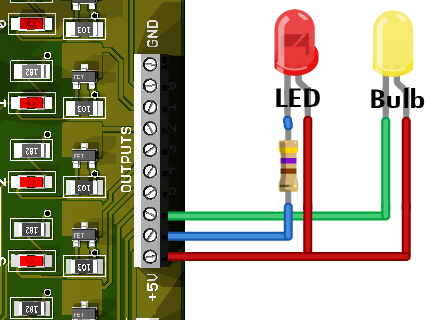
\includegraphics[width=3in]{images/Outputs-indicator.png}
\caption{Wiring LEDs and bulbs to Io output}
\label{indicators}
\end{center}
\end{figure}

\section{Usage Example: Digitrax DS64 Quad Stationary Decoder}

TODO image of screw terminals and DS64

\section{Usage Example: NCE TODO}

\chapter{Configuring Railstars Io}

TODO images of b/g buttons and LEDs

\chapter{Using the TCH Technology OpenLCB USB/CAN Interface to connect your PC}

TODO image of USB interface

\chapter{Advanced Topic: Writing custom firmware for Railstars Io}

\section{Connecting the USB adapter}
\label{FTDI}


%%%%%%%%%%%%%%%%%%%%
%end matters

\printindex

\newpage
Figures \ref{DPDT}, \ref{pushbutton}, TODO were created with Fritzing. \url{http://fritzing.org/}

Railstars\texttrademark and Io\texttrademark are trademarks of Railstars Limited. TCH Technology\texttrademark is a trademark of Timothy C. Hatch. NMRA\texttrademark, is a trademark of, and NMRAnet\textregistered and the NMRAnet logo are registered trademarks of the National Model Railroading Association.

TODO Digitrax, NCE

\end{document}  